\documentclass[twocolappendix, appendixfloats, numberedappendix, twocolumn, apj]{openjournal}

\usepackage{graphicx}
\usepackage{latexsym,amssymb}
\usepackage{amsmath,morefloats}
\usepackage[backref,breaklinks,colorlinks,citecolor=blue]{hyperref}
\usepackage{natbib,graphicx,amsmath,subfigure,color,xcolor}
\usepackage{verbatim}
\usepackage{threeparttable}
\usepackage{xspace}

\newcommand{\ess}[1]{\textcolor{red}{[ESS: \bf #1]}\xspace}
\newcommand{\mrb}[1]{\textcolor{purple}{[MRB: \bf #1]}\xspace}

\newcommand{\mdet}{\textsc{metadetection}\xspace}
\newcommand{\mcal}{\textsc{metacalibration}\xspace}
\newcommand{\galsim}{\textsc{galsim}\xspace}
\newcommand{\descwl}{\textsc{WeakLensingDeblending}\xspace}
\newcommand{\ngmix}{\textsc{ngmix}\xspace}
\newcommand{\sep}{\textsc{sep}\xspace}

\shorttitle{\mdet with coadding}
\shortauthors{Becker, Sheldon \& Jarvis}

\begin{document}
\title{Metadetection in Multi-Epoch Surveys: Algorithms for Image Coaddition and Pixel-Level Artifact Correction}

\author{Matthew R. Becker}
\affil{High Energy Physics Division, Argonne National Laboratory, Lemont, IL 60439, USA}
\author{Erin S. Sheldon}
\affil{Brookhaven National Laboratory, Bldg 510, Upton, New York 11973, USA}
\author{Michael Jarvis}
\affil{Department of Physics and Astronomy, University of Pennsylvania, Philadelphia, PA 19104, USA}


\begin{abstract}
\mdet is a promising technique for making weak gravitational lensing measurements in the presence of
object detection and blending. Currently published tests of this algorithm were only done in
highly idealized situations, neglecting the effects of pixel-level artifact masking, image edges,
and image coaddition through world coordinate system transforms. In this work, we develop algorithms
to address each of these effects and demonstrate that \mdet weak lensing shear measurements are
unbiased to better than 0.1\% even in the presence of these effects. Looking forward, this work provides
a baseline set of algorithms that can be implemented in the analysis pipelines of real surveys.
Future challenges remain, especially concerning image background subtraction, the handling of bright stars,
and techniques to join \mdet measurements across different survey patches. Ongoing work in current-
and next-generation surveys will test these techniques and potentially bring yet unknown issues to light.
\end{abstract}


\section{Introduction}\label{sec:intro}

\section{Weak Lensing \& \mdet}\label{sec:background}

\section{Methodology and Simulations}\label{sec:sims}

\subsection{Image Interpolation and Coadding Procedures}\label{sec:coadd}

\mdet's defining feature is the re-detection of sources in each of the \mcal
sheared images. This procedure constrains possible algorithms for implementing
\mdet in real surveys in several ways.

\begin{itemize}
  \item The regions over which we apply \mdet
  must be big enough that detection algorithms run correctly.
  \item As \mcal requires deconvolving the PSF, the regions we use must not have
  single-epoch image edges and or missing pixels for some of the input images. These features
  would result in PSF discontinuities.
  \item The PSF of the resulting coadd must be computable from the input image PSFs.
  \item A sample of the noise correlation field must be computable from the input images.
  This noise sample is used to cancel the effects of the sheared noise generated
  by the \mcal process.
  \item Variable PSF deconvolutions, while possible, are numerically expensive, so the input
  region must be small enough that we can safely neglect any residual PSF variation in the coadd image.
\end{itemize}

While the constraint that we need to apply detection algorithms to the coadd argues
for larger coadd regions, the constraint that we need an exact, constant, computable
PSF for the resulting coadd image argues for smaller coadd regions. This last constraint is
particularly an issue for modern surveys where the gaps between CCDs on the focal plane
combined with semi-structured tilling make finding a large, CCD edge-free region difficult
if not impossible to find. Ultimately, the size of the coadd region will be compromise
between these different things and will greatly depend on the details of a given survey.
With these considerations in mind, we target our tests at coadd regions of about 1 arcminute
on a side, which appear to be close to optimal for an LSST-like survey \citep{ArmstrongCoadd}.

\begin{figure*}
    \begin{center}
        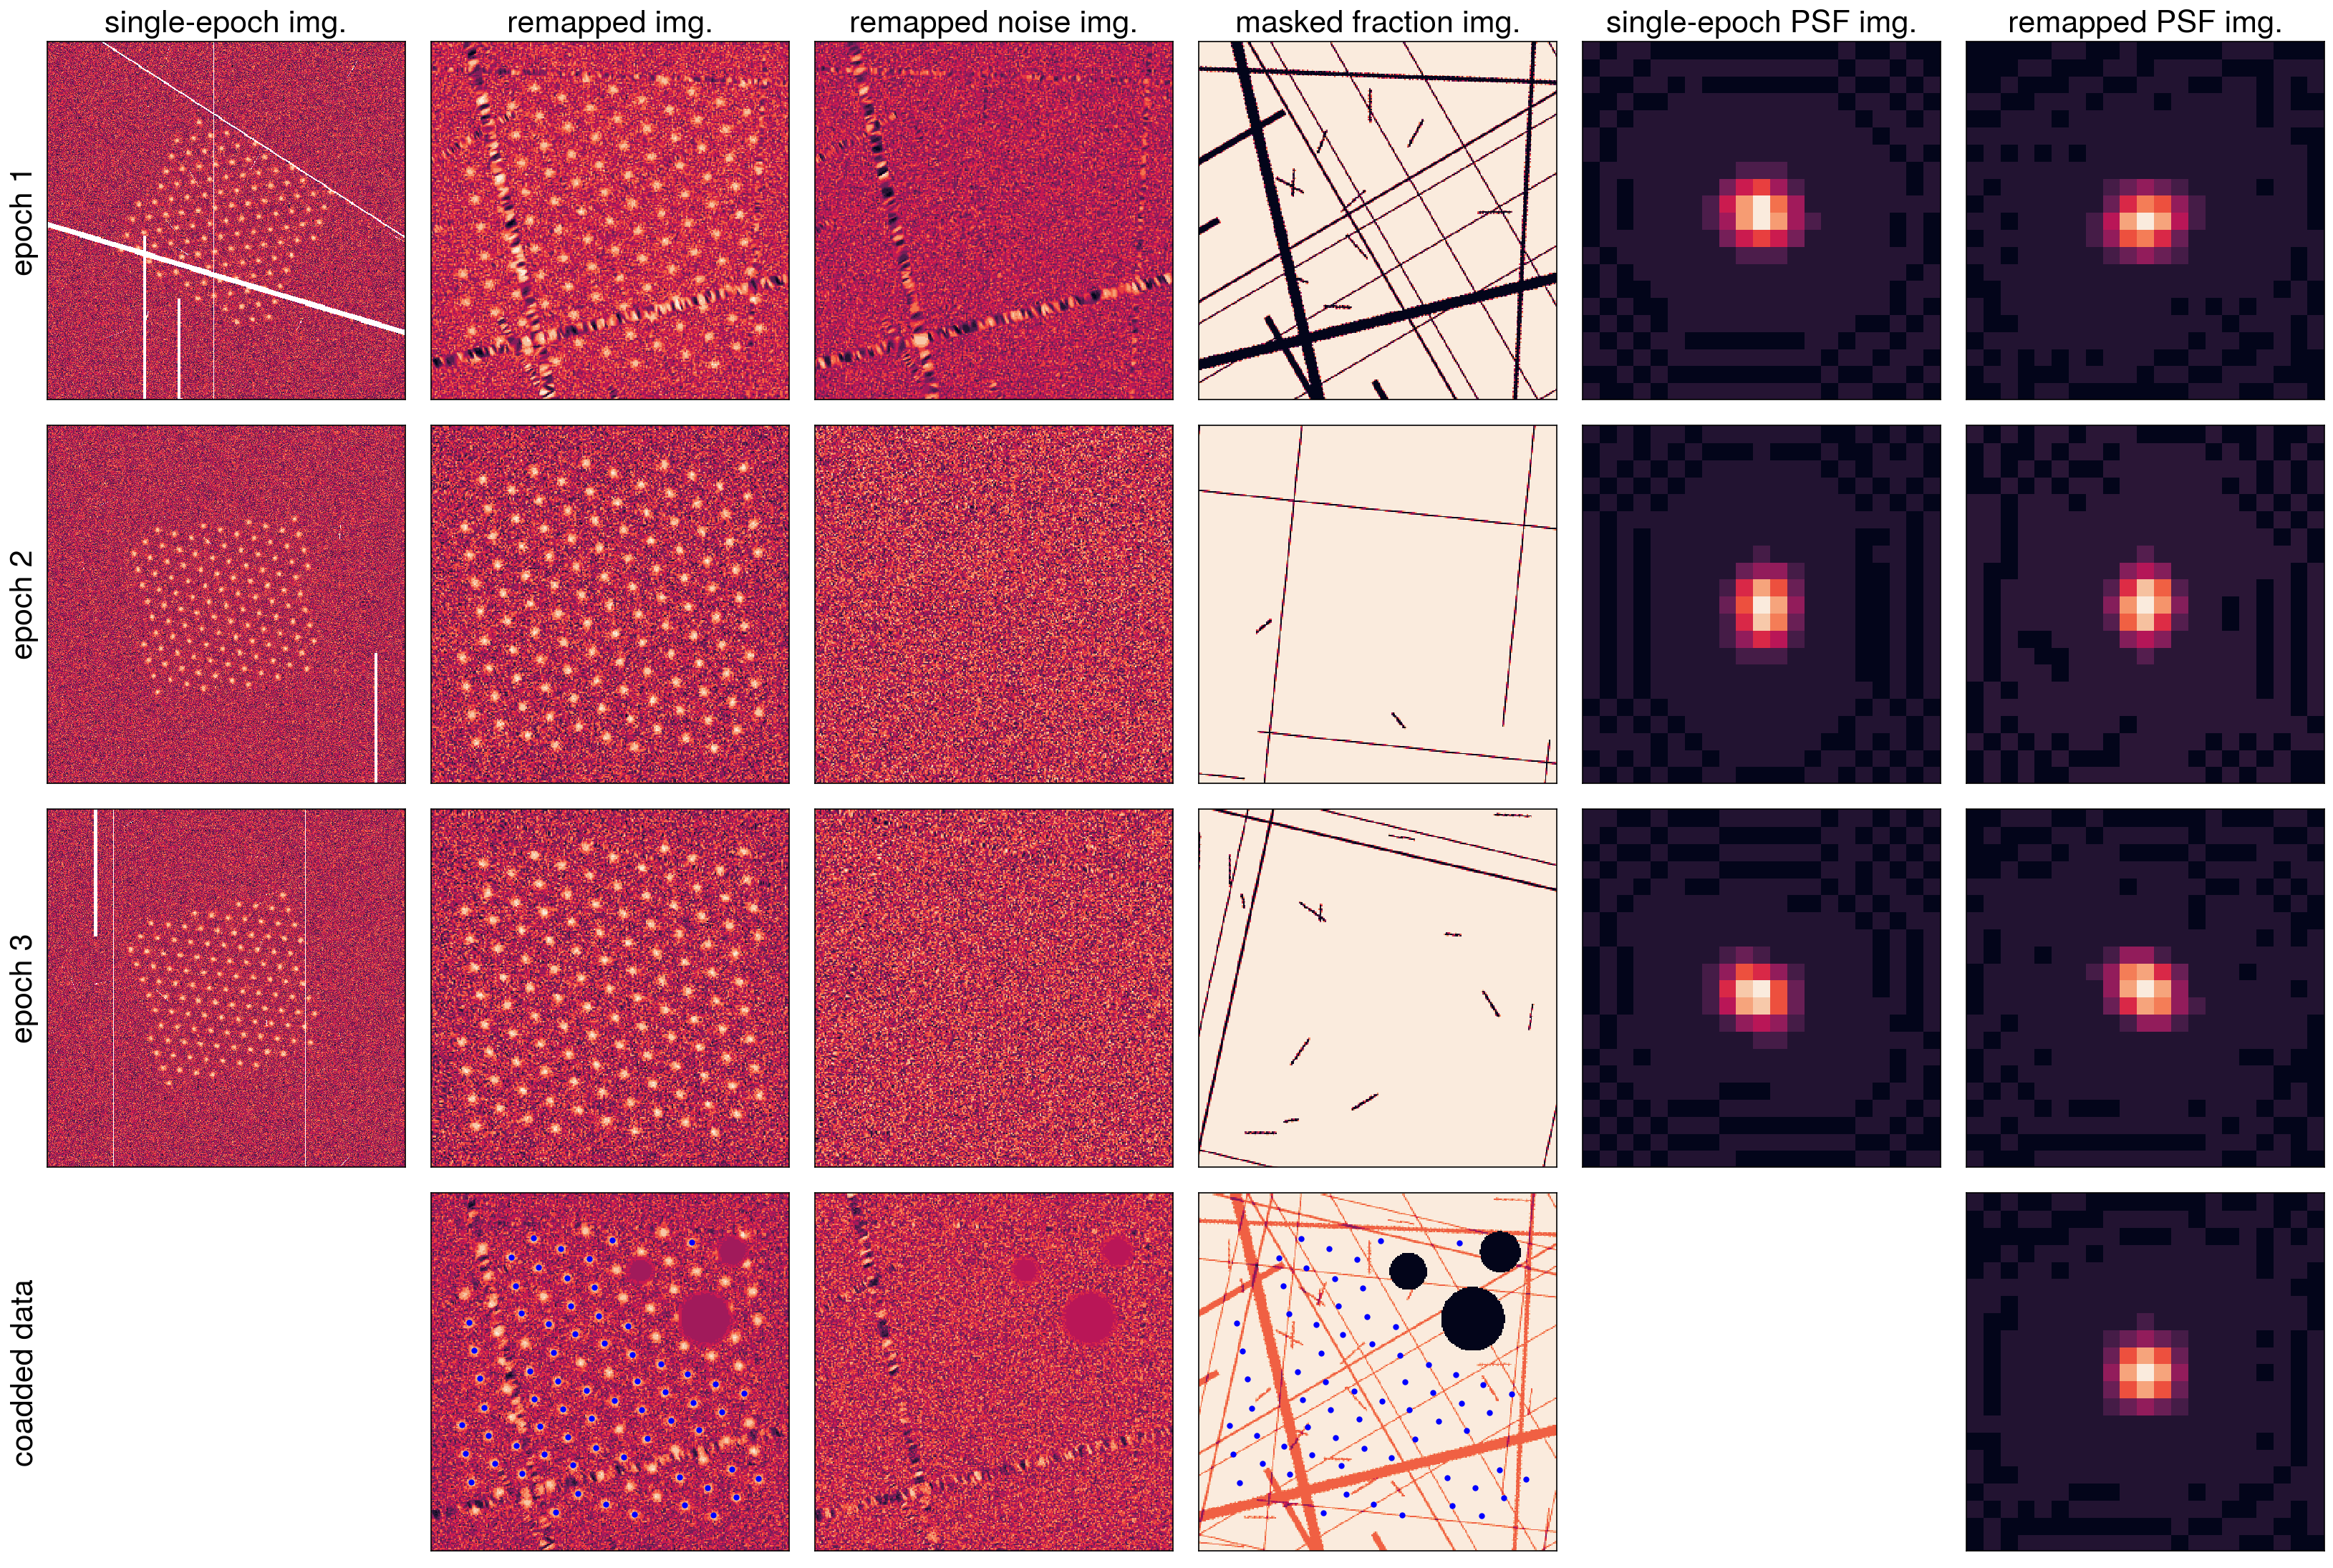
\includegraphics[width=\textwidth]{allsteps.png}
        \caption{\label{fig:allsteps}}
    \end{center}
\end{figure*}

Given the target size of the coadd region, one must choose a suitable projection
and pixel scale for the coadd coordinate system. With this choice, the coadding process
works as follows (see Figure~\ref{fig:allsteps}):

\begin{enumerate}
\item Find every single-epoch that completely contains within its boundaries the entire coadd region.
\item Find the pixel center closest to the center of the coadd region, defined here as the coadd center.
\item For each of these single-epoch images:
\begin{enumerate}
  \item Generate a noise realization with the same pixel noise correlations.
  \item Interpolate all pixels with missing data in the image.
  \item Apply the same interpolation algorithm to the same pixels in the generated noise image.
  \item Compute the location of the coadd center in the single-epoch image coordinates.
  \item Generate an image of the PSF at the location of the coadd center in the single-epoch image coordinates.
  \item Construct a masked fraction map for the single-epoch image which marks the fraction of each pixel
  which was interpolated (i.e., either 0 or 1 in this case).
  \item Resample the image, the noise image, the PSF image, and the masked fraction image to the coadd coordinate system.
\end{enumerate}
\item Using the resampled single-epoch data products from the last step, form a (possibly weighted) coadd image
by summing them together with an appropriately normalized set of weights.
\end{enumerate}
For image interpolation, we use a \mrb{describe} in the \texttt{scipy} package \citep{scipy}. For image resampling,
we use a Lanczos-3 interpolation as a compromise between optimally resampling the image and artificially
smoothing the image more than needed. In real survey processing, one usually keeps bit masks indicating
processing steps done on each pixel. Those too can be propagated through these steps. One very important
feature of this algorithm is where we draw the PSF. By drawing the PSF at the single-epoch location for each
image that corresponds to the same location in the coadd coordinate system, we properly track how the resampling
process slightly broadens the PSF in the final coadd. Further, by putting pure noise images through the same
coadding process, we automatically generate a noise image with the proper noise correlations in the final coadd.
This noise image is needed by \mcal, as described above. Finally, we show below that by measuring the weighted
amplitude of the coadd masked fraction image at each detection center, we can incorporate a masked fraction cut
into \mdet that helps to reject objects with excessively interpolated flux.

\subsection{Simulations and Pixel-level Artifact Generation}

\begin{figure}
    \begin{center}
        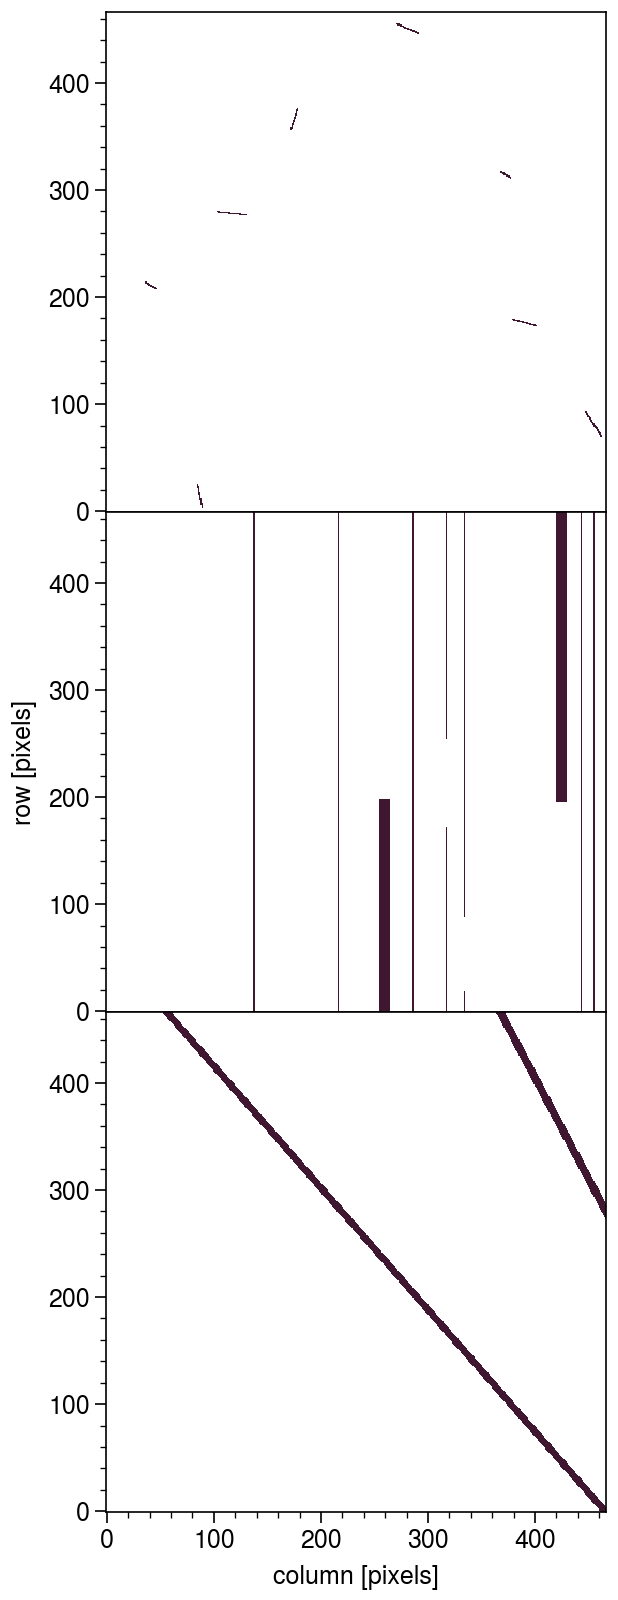
\includegraphics[width=0.75\columnwidth]{masking.png}
        \caption{\label{fig:mcgen}}
    \end{center}
\end{figure}

\mrb{put in final numbers for various things like PSF params, cosmics density, bad columns, etc.}

We use simulations based on those in \citet{mdet} to test the interpolation and coadding algorithms
discussed in Section~\ref{sec:coadd}. We use the \galsim package \citep{GALSIM2015} to simulate
objects based on either simple exponential profiles or based on the \descwl package
\citep{WeakLensingDeblendingPaper,WeakLensingDeblendingSoftware}. Following \citet{mdet}, we apply a constant shear
to our simulations, shearing the entire field of view including the object positions. Each simulated coadd patch is
275 coadd pixels on a side with objects only drawn if their center falls in the central 225 pixels. This coadd coordinate
system is completely flat with a pixel scale of 0.263 arcseconds. We simulate one or more single-epoch images that overlap this
coadd coordinate system and then use the algorithms above to form the coadd image from which we measure shear.
Our simulation code is available publicly online.\footnote{\url{https://github.com/beckermr/pizza-cutter-sims}}

One key change in the simulations in this work is the inclusion of pixel-level artifacts and non-trivial
WCS' for the images. For this task, we have written a series of Monte Carlo generators. They generate
cosmic ray-like defects, bad column-like defects, large rectangular areas which are completely masked (e.g.,
bad amplifiers or masked bleeds), and satellite streak-like defects \mrb{finish this in the sims}. Bad pixel
masks from these various generators are illustrated in Figure~\ref{fig:mcgen}. We have adjusted the rates
of these defects to be typical for modest length exposure in a ground-based survey like the Dark energy Survey
\citep{des}.

Our non-trivial WCS transformations are generated by drawing a subpixel offset relative to the coadd WCS,
generating a different pixel scale, and generating a small shear applied to the coordinates. In this work, we focus on
surveys where the single-epoch coordinate systems have extremely small or zero position angles relative to the
coadd coordinate system. Such geometries are generated by telescopes on equatorial mounts with no ability to rotate the
camera about the center of the field of view. The effects of position angle rotation on the algorithms
here will be explored in future work, currently in preparation \citep{sheldoninprep}.

Finally, we generate PSFs either assuming a Gaussian model with varying widths and shapes
per single-epoch image or by using the power-spectrum model from \citep{mdet}. \mrb{describe this more}.

\subsection{Simulation Analysis}

We use the \mdet algorithm to measure the shear in our simulations. The \mdet algorithm is implemented in
\ngmix and uses the \sep package \citep{sep} for detection. We use a weighted Gaussian moment for the shape
measurement with a full-width at half-maximum of 1.2 arcseconds. We also measure the mean masked fraction
of each object weighted by the same aperture as the shape measurement. We employ cuts on the object area relative to
the PSF area, the object signal to noise, and the weighted masked fraction.

To make our simulations more efficient, we employ the noise cancellation method from \citet{pujol2019}. In this technique,
we generate the same simulation with the same pixel noise, defects, objects etc., but change the sign of
the shear. We then subtract the mean shape estimates from each simulation, which results in a cancellation of
the pixel noise while retaining the shear signal.

We characterize the results the results of our simulations by the standard multiplicative ($m$) and additive ($c$) biases
\begin{equation}
g_{obs} = (1+m)g_{true} + c\ .
\end{equation}
Our final errors on these quantities are computed by bootstrapping over a the mean shape estimate from large
number of simulated patches.

\section{Results}\label{sec:results}

\subsection{Small-area Masking Effects and WCS Variations}

\begin{table*}
  \centering
  \begin{threeparttable}
  \caption{
    Multiplicative and additive biases in weak lensing simulations for various simulation
    configurations.}
  \label{tab:shearmeas}

  \begin{tabular}{lcccc}
    \hline
    \noalign{\vskip 1mm}
    Survey & Sim (\texttt{WCS-gals-msk-PSF})\tnote{1} & \# of SE images & m [$10^{-3}$ $3\sigma$ error] & c [$10^{-5}$ $3\sigma$ error]\\
    \noalign{\vskip 1mm}
    \hline
    \noalign{\vskip 1mm}
    bright exp. & \texttt{d-g-None-gf} & 1 & $0.43 \pm 0.18$ & $0.072 \pm 0.438$ \\
    dim exp. & \texttt{None-g-rct-gf} & 1 & $-0.19 \pm  0.30$ & $ 0.11 \pm  0.55$ \\
    \noalign{\vskip 1mm}
    \hline
  \end{tabular}

  \begin{tablenotes}
  \item [1] description goes here
  \end{tablenotes}
  \end{threeparttable}
\end{table*}


\subsection{Response Computations Across Big-area Mask Edges}

In addition to the small-area pixel-level artifacts we tested above, realistic surveys will have a variety of
larger-area masked regions which are fixed on the sky. These will be mainly due to bright stars in our own galaxy,
but might also include large, nearby galaxies which are not useful for weak lensing at cosmological distances. These areas,
because they are fixed on the sky, present special challenges for weak lensing and \mdet in particular. Unlike the small-area features
that are randomly located on the single-epoch images, we cannot hope to interpolate properly in these regions both because of their size and
because these regions pile up in the same location in the final coadd images. Furthermore, we do
not have access to the data in the masked regions. Thus, when we generate the sheared images in the \mdet process, we cannot
properly simulate how the shape measurements of objects near the mask edges change because we cannot measure any extra part of
the image that would have not been masked under a slightly different shear.

We propose the following procedure to correctly compute the response in these cases. A fiducial mask is applied to the data before
the \mdet process. This mask is applied to help control artifacts in the \mdet simulation process itself due to bright stars
and other numerical effects as discussed in \citep{sheldoninprep}. We then interpolate these masked regions and create the five
\mdet images. Finally, we apply a slightly larger version of the mask where the masked area has been increased by a small amount
along the boundaries. This amount should be big enough to capture the changes in objects' profiles as they are sheared. An
increase of a few arcseconds or $\sim10$ pixels for a DES-like survey should be sufficient. We then measure the shear and
response as usual. This procedure uses a small amount of image area around masked regions to properly simulate how objects near a
mask edge change under shear with the effects of masking.

Before testing this procedure directly, we demonstrate that if we had access to the imaging behind the masked regions, \mdet would work
correctly given modest cuts on objects which are too heavily masked. For this test, we directly simulate the five different \mdet images
and apply a fixed mask of randomly placed star-like holes to each one. We reject any objects with a masked pixel within the eight central pixels around the object's center. In this case, for bright exponential objects with a Gaussian PSF on a grid, we find $m=0.29 \pm 0.29 [10^{-3}, 3\sigma]$ \mrb{put in numbers for 4 pixels} consistent with the expectations from second-order shear effects. This test indicates that indeed the edge effects can be corrected by \mdet if we have access to the data behind the mask.


\section{Summary}\label{sec:conc}

\section*{Acknowledgments}

ESS is supported by DOE grant DE-AC02-98CH10886, and MRB is supported by DOE
grant DE-AC02-06CH11357.  We gratefully acknowledge the computing resources
provided on Bebop, a high-performance computing cluster operated by the
Laboratory Computing Resource Center at Argonne National Laboratory, and the
RHIC Atlas Computing Facility, operated by Brookhaven National Laboratory.
This work also used resources made available on the Phoenix cluster, a joint
data-intensive computing project between the High Energy Physics Division and
the Computing, Environment, and Life Sciences (CELS) Directorate at Argonne
National Laboratory.

\bibliographystyle{aasjournal}
\bibliography{references}

% \appendix

\end{document}
